\documentclass{article}
%--PASTE INTO MAIN FILE--
% \documentclass{article}
% %--PASTE INTO MAIN FILE--
% \documentclass{article}
% %--PASTE INTO MAIN FILE--
% \documentclass{article}
% \input{TexBase/DocumentBase.tex}
% \end{document}

\usepackage[margin = 0.7in]{geometry}
\usepackage{graphicx}
\usepackage{graphics}
\usepackage[T1]{fontenc}
\usepackage[polish]{babel}
\usepackage{cmap}
\usepackage[utf8]{inputenc}
\usepackage{float}
\usepackage{tabularx}
\usepackage[table,xcdraw]{xcolor}
\usepackage{lipsum}
\usepackage{titlesec}
\usepackage{minted}
\usepackage{xcolor}
\usepackage{caption}
\usepackage{enumitem}
\usepackage{csvsimple}
\usepackage{natbib}
\usepackage{blindtext}

\usepackage{amsmath} %math

\usepackage{numprint} % rounding
\usepackage[round-precision=3,round-mode=figures, scientific-notation=true]{siunitx} %scientific notation

\usepackage[hidelinks]{hyperref}
\usepackage{url}

\usepackage{bm} %bold for math


%TABS
\usepackage[]{booktabs}
\usepackage{tabularray}
\usepackage{multirow}

%\title{}
\author{Michał Dziedziak}
\date{\today}


\titlespacing\section{0pt}{12pt plus 4pt minus 2pt}{0pt plus 2pt minus 2pt}
\titlespacing\subsection{0pt}{12pt plus 4pt minus 2pt}{0pt plus 2pt minus 2pt}
\titlespacing\subsubsection{0pt}{12pt plus 4pt minus 2pt}{0pt plus 2pt minus 2pt}
\setlength{\parskip}{\baselineskip}%
\setlength{\parindent}{0pt}%

\newcommand{\squeezeup}{\vspace{-5mm}}


\begin{document}

\begin{titlepage}
    \begin{center}
        \vspace*{5cm}
        \rule{500pt}{1pt}\\
        \vspace*{0.5cm}
        \LARGE
        \textbf{Inżyniera Obrazów}\\
        \Large
        Laboratorium numer 2
        \vspace*{0.5cm}
        \rule{500pt}{1pt}
    \end{center}

    \vspace*{10cm}

    {\raggedright
        \large
        \textbf{Autor sprawozdania:} Michał Dziedziak 263901\\
        \textbf{Imię i Nazwisko prowadzącego kurs:} dr inż. Jan Nikodem\\
        \textbf{Dzień i godzina zajęć:} czwartek, 11:15 - 14:15
    }
\end{titlepage}


\tableofcontents
% \listoftables

%\renewcommand\listoflistingscaption{List of source codes}
% \listoflistings

\listoffigures


\newpage


% \begin{table}[H]
%     \centering
%     \begin{tabular}{|c|c|c|c|}%
%         \hline
%         \bfseries Numer iteracji & \bfseries Czas zalezienia rozwiązania [ms] & Koszt ścieżki & Błąd względny% specify table head
%         \csvreader[head to column names]{Csv/BestPathTest_SimulatedAnnealing_LINEAR_ftv47.csv}{}% use head of csv as column names
%         {\\\hline\Iteration & \num{\TimeInMiliSeconds} & \Cost & \num[round-precision=2, round-mode=places, scientific-notation=false]{\Error}\%}% specify your columns here
%         \\\hline    
%     \end{tabular}
%     \caption{}
%     \label{tab:}
% \end{table}

% \begin{figure}[H]
%     \centering
%     \resizebox{\columnwidth}{!}{%
%     \includegraphics{}%
%     }
%     \caption{}
%     \label{fig:}
% \end{figure}

% \begin{listing}[H]
%     \begin{minted}[frame=single,framesep=2mm,linenos,fontsize=\footnotesize]{language}
%         some code
%     \end{minted}
%     \caption{}
%     \label{lst:}
% \end{listing}


% \bibliographystyle{plainnat}
% \bibliography{TexBase/Bibliography}

% \end{document}

\usepackage[margin = 0.7in]{geometry}
\usepackage{graphicx}
\usepackage{graphics}
\usepackage[T1]{fontenc}
\usepackage[polish]{babel}
\usepackage{cmap}
\usepackage[utf8]{inputenc}
\usepackage{float}
\usepackage{tabularx}
\usepackage[table,xcdraw]{xcolor}
\usepackage{lipsum}
\usepackage{titlesec}
\usepackage{minted}
\usepackage{xcolor}
\usepackage{caption}
\usepackage{enumitem}
\usepackage{csvsimple}
\usepackage{natbib}
\usepackage{blindtext}

\usepackage{amsmath} %math

\usepackage{numprint} % rounding
\usepackage[round-precision=3,round-mode=figures, scientific-notation=true]{siunitx} %scientific notation

\usepackage[hidelinks]{hyperref}
\usepackage{url}

\usepackage{bm} %bold for math


%TABS
\usepackage[]{booktabs}
\usepackage{tabularray}
\usepackage{multirow}

%\title{}
\author{Michał Dziedziak}
\date{\today}


\titlespacing\section{0pt}{12pt plus 4pt minus 2pt}{0pt plus 2pt minus 2pt}
\titlespacing\subsection{0pt}{12pt plus 4pt minus 2pt}{0pt plus 2pt minus 2pt}
\titlespacing\subsubsection{0pt}{12pt plus 4pt minus 2pt}{0pt plus 2pt minus 2pt}
\setlength{\parskip}{\baselineskip}%
\setlength{\parindent}{0pt}%

\newcommand{\squeezeup}{\vspace{-5mm}}


\begin{document}

\begin{titlepage}
    \begin{center}
        \vspace*{5cm}
        \rule{500pt}{1pt}\\
        \vspace*{0.5cm}
        \LARGE
        \textbf{Inżyniera Obrazów}\\
        \Large
        Laboratorium numer 2
        \vspace*{0.5cm}
        \rule{500pt}{1pt}
    \end{center}

    \vspace*{10cm}

    {\raggedright
        \large
        \textbf{Autor sprawozdania:} Michał Dziedziak 263901\\
        \textbf{Imię i Nazwisko prowadzącego kurs:} dr inż. Jan Nikodem\\
        \textbf{Dzień i godzina zajęć:} czwartek, 11:15 - 14:15
    }
\end{titlepage}


\tableofcontents
% \listoftables

%\renewcommand\listoflistingscaption{List of source codes}
% \listoflistings

\listoffigures


\newpage


% \begin{table}[H]
%     \centering
%     \begin{tabular}{|c|c|c|c|}%
%         \hline
%         \bfseries Numer iteracji & \bfseries Czas zalezienia rozwiązania [ms] & Koszt ścieżki & Błąd względny% specify table head
%         \csvreader[head to column names]{Csv/BestPathTest_SimulatedAnnealing_LINEAR_ftv47.csv}{}% use head of csv as column names
%         {\\\hline\Iteration & \num{\TimeInMiliSeconds} & \Cost & \num[round-precision=2, round-mode=places, scientific-notation=false]{\Error}\%}% specify your columns here
%         \\\hline    
%     \end{tabular}
%     \caption{}
%     \label{tab:}
% \end{table}

% \begin{figure}[H]
%     \centering
%     \resizebox{\columnwidth}{!}{%
%     \includegraphics{}%
%     }
%     \caption{}
%     \label{fig:}
% \end{figure}

% \begin{listing}[H]
%     \begin{minted}[frame=single,framesep=2mm,linenos,fontsize=\footnotesize]{language}
%         some code
%     \end{minted}
%     \caption{}
%     \label{lst:}
% \end{listing}


% \bibliographystyle{plainnat}
% \bibliography{TexBase/Bibliography}

% \end{document}

\usepackage[margin = 0.7in]{geometry}
\usepackage{graphicx}
\usepackage{graphics}
\usepackage[T1]{fontenc}
\usepackage[polish]{babel}
\usepackage{cmap}
\usepackage[utf8]{inputenc}
\usepackage{float}
\usepackage{tabularx}
\usepackage[table,xcdraw]{xcolor}
\usepackage{lipsum}
\usepackage{titlesec}
\usepackage{minted}
\usepackage{xcolor}
\usepackage{caption}
\usepackage{enumitem}
\usepackage{csvsimple}
\usepackage{natbib}
\usepackage{blindtext}

\usepackage{amsmath} %math

\usepackage{numprint} % rounding
\usepackage[round-precision=3,round-mode=figures, scientific-notation=true]{siunitx} %scientific notation

\usepackage[hidelinks]{hyperref}
\usepackage{url}

\usepackage{bm} %bold for math


%TABS
\usepackage[]{booktabs}
\usepackage{tabularray}
\usepackage{multirow}

%\title{}
\author{Michał Dziedziak}
\date{\today}


\titlespacing\section{0pt}{12pt plus 4pt minus 2pt}{0pt plus 2pt minus 2pt}
\titlespacing\subsection{0pt}{12pt plus 4pt minus 2pt}{0pt plus 2pt minus 2pt}
\titlespacing\subsubsection{0pt}{12pt plus 4pt minus 2pt}{0pt plus 2pt minus 2pt}
\setlength{\parskip}{\baselineskip}%
\setlength{\parindent}{0pt}%

\newcommand{\squeezeup}{\vspace{-5mm}}


\begin{document}

\begin{titlepage}
    \begin{center}
        \vspace*{5cm}
        \rule{500pt}{1pt}\\
        \vspace*{0.5cm}
        \LARGE
        \textbf{Inżyniera Obrazów}\\
        \Large
        Laboratorium numer 2
        \vspace*{0.5cm}
        \rule{500pt}{1pt}
    \end{center}

    \vspace*{10cm}

    {\raggedright
        \large
        \textbf{Autor sprawozdania:} Michał Dziedziak 263901\\
        \textbf{Imię i Nazwisko prowadzącego kurs:} dr inż. Jan Nikodem\\
        \textbf{Dzień i godzina zajęć:} czwartek, 11:15 - 14:15
    }
\end{titlepage}


\tableofcontents
% \listoftables

%\renewcommand\listoflistingscaption{List of source codes}
% \listoflistings

\listoffigures


\newpage


% \begin{table}[H]
%     \centering
%     \begin{tabular}{|c|c|c|c|}%
%         \hline
%         \bfseries Numer iteracji & \bfseries Czas zalezienia rozwiązania [ms] & Koszt ścieżki & Błąd względny% specify table head
%         \csvreader[head to column names]{Csv/BestPathTest_SimulatedAnnealing_LINEAR_ftv47.csv}{}% use head of csv as column names
%         {\\\hline\Iteration & \num{\TimeInMiliSeconds} & \Cost & \num[round-precision=2, round-mode=places, scientific-notation=false]{\Error}\%}% specify your columns here
%         \\\hline    
%     \end{tabular}
%     \caption{}
%     \label{tab:}
% \end{table}

% \begin{figure}[H]
%     \centering
%     \resizebox{\columnwidth}{!}{%
%     \includegraphics{}%
%     }
%     \caption{}
%     \label{fig:}
% \end{figure}

% \begin{listing}[H]
%     \begin{minted}[frame=single,framesep=2mm,linenos,fontsize=\footnotesize]{language}
%         some code
%     \end{minted}
%     \caption{}
%     \label{lst:}
% \end{listing}


% \bibliographystyle{plainnat}
% \bibliography{TexBase/Bibliography}



\section{Zadanie pierwsze}
    \subsection{Cel ćwiczenia}
    Zadanie pierwsze polegało na zastosowaniu filtru górnoprzepustowego (tzw. detektora krawędzi) do obrazu. 
    W tym celu mieliśmy wykorzystać maskę:
    \[
        \begin{bmatrix}
            -1 & -1 & -1 \\
            -1 & 8 & -1 \\
            -1 & -1 & -1
        \end{bmatrix}
    \]

    \subsection{Teoria}
    Filtry obrazów są kluczowym narzędziem w dziedzinie przetwarzania obrazów, 
    służącym do modyfikacji wyglądu i charakterystyk obrazu poprzez różnorodne operacje matematyczne 
    na pikselach. Wśród podstawowych rodzajów filtrów wyróżnia się filtry górnoprzepustowe i dolnoprzepustowe.

    Filtry górnoprzepustowe, takie jak implementowany w zadaniu filtr Laplace'a, mają za zadanie podkreślać detale i krawędzie
    poprzez eliminację niskoczęstotliwościowych składowych obrazu i przepuszczanie wysokoczęstotliwościowych. 
    Działają na zasadzie mnożenia wartości pikseli przez odpowiednie współczynniki z maski, 
    co prowadzi do wyostrzenia obrazu i podkreślenia struktur. 
    
    Przykładowe filtry górnoprzepustowe to
    \begin{itemize}
        \item Filtr Laplace'a
        \item Filtr usuń średnią (ang. mean removal)
        \item Filtr HP1, HP2, HP3
    \end{itemize}

    
    Z kolei filtry dolnoprzepustowe, np. filtr Gaussa, przepuszczają składowe niskoczęstotliwościowe, 
    eliminując wysokoczęstotliwościowe. Ich działanie polega na wygładzaniu obrazu poprzez średnią lub 
    ważoną wartość pikseli w otoczeniu. W efekcie uzyskuje się efekt rozmycia, który może być wykorzystywany 
    m.in. do redukcji szumów.

    Przykładowe filtry dolnoprzepustowe to
    \begin{itemize}
        \item Filtr uśredniający
        \item Filtr kołowy
        \item Filtr piramidalny
    \end{itemize}
        
    Źródło: \cite{Lubinski2007}

    \subsection{Prezentacja wykonanego zadania}
    \begin{figure}[H]
        \centering
        \resizebox{\columnwidth}{!}{%
        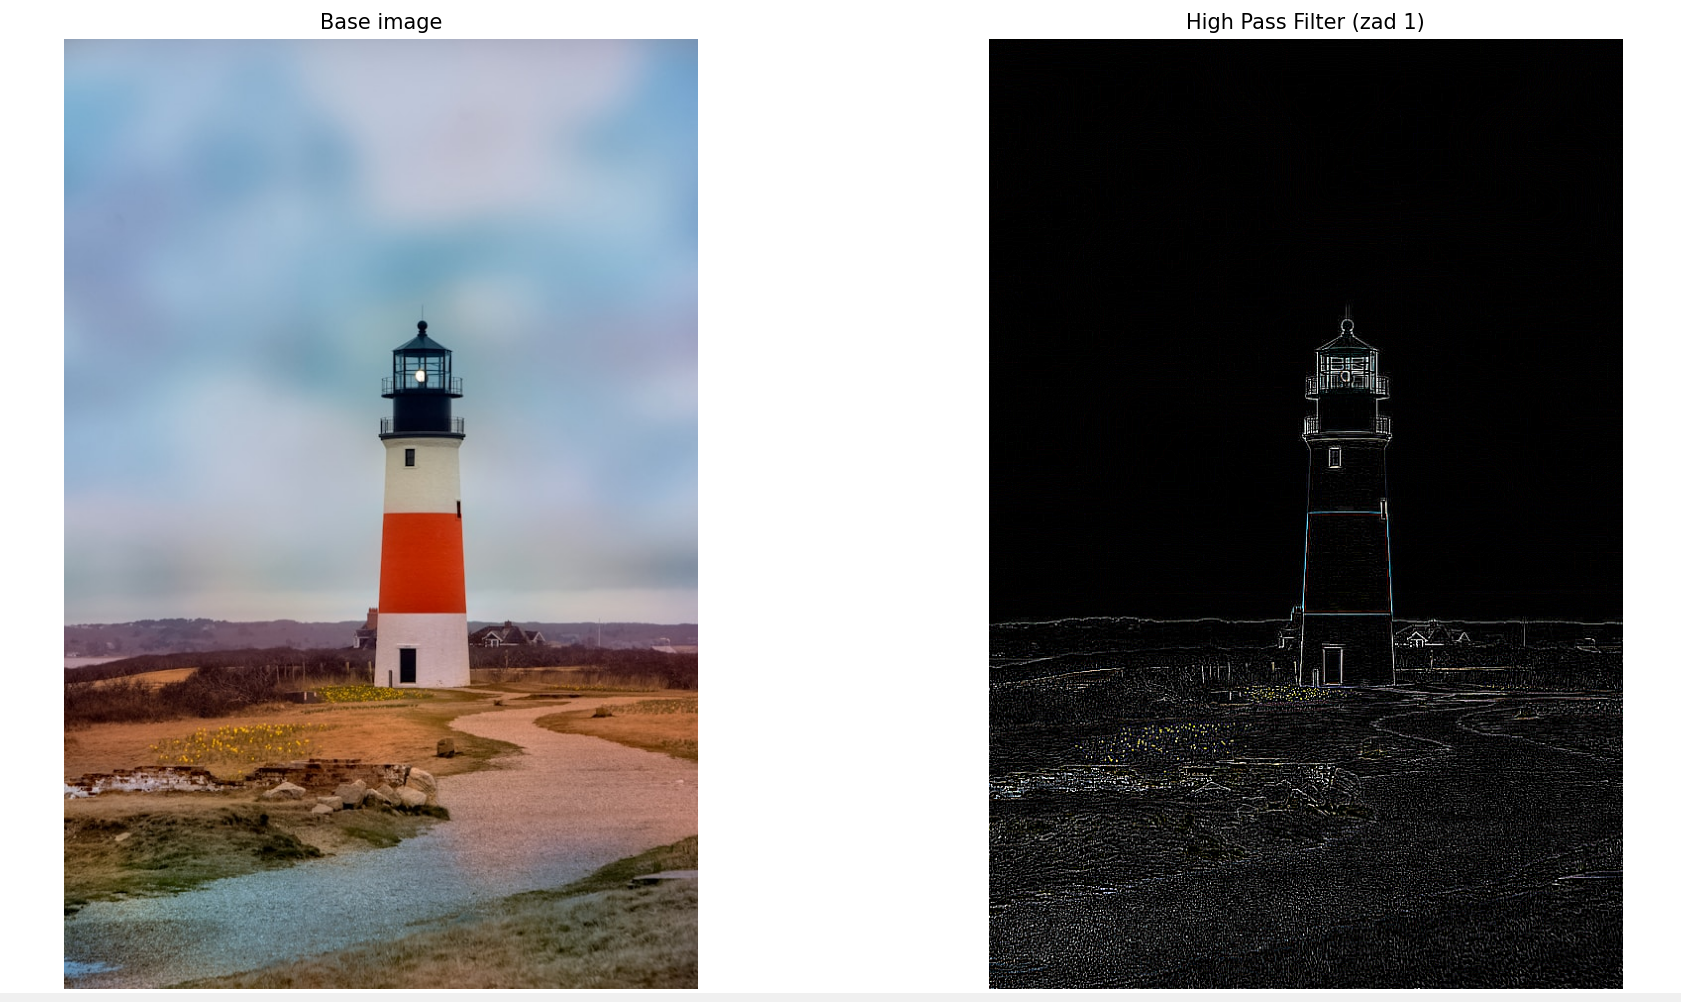
\includegraphics{Img/zad1.png}%
        }
        \caption{Zdjęcie oryginalne i po nałożeniu filtru górnoprzepustowego podanego w zadaniu}
    \end{figure}

    \subsection{Wizualizację wybranych filtrów}


    \subsection{Eksperymenty z modyfikacją maski}

    \begin{enumerate}
        \item Obraz dla maski $\begin{bmatrix}
                                    1 & 1 & 1 \\
                                    1 & 8 & 1 \\
                                    1 & 1 & 1
                                \end{bmatrix}$
        \item Obraz dla maski $\begin{bmatrix}
                                    0 & 1/21 & 1/21 & 1/21 & 0 \\
                                    1/21 & 1/21 & 1/21 & 1/21 & 1/21 \\
                                    1/21 & 1/21 & 1/21 & 1/21 & 1/21 \\
                                    1/21 & 1/21 & 1/21 & 1/21 & 1/21 \\
                                    0 & 1/21 & 1/21 & 1/21 & 0
                                \end{bmatrix}$
    \end{enumerate}

    \begin{figure}[H]
        \centering
        \resizebox{\columnwidth}{!}{%
        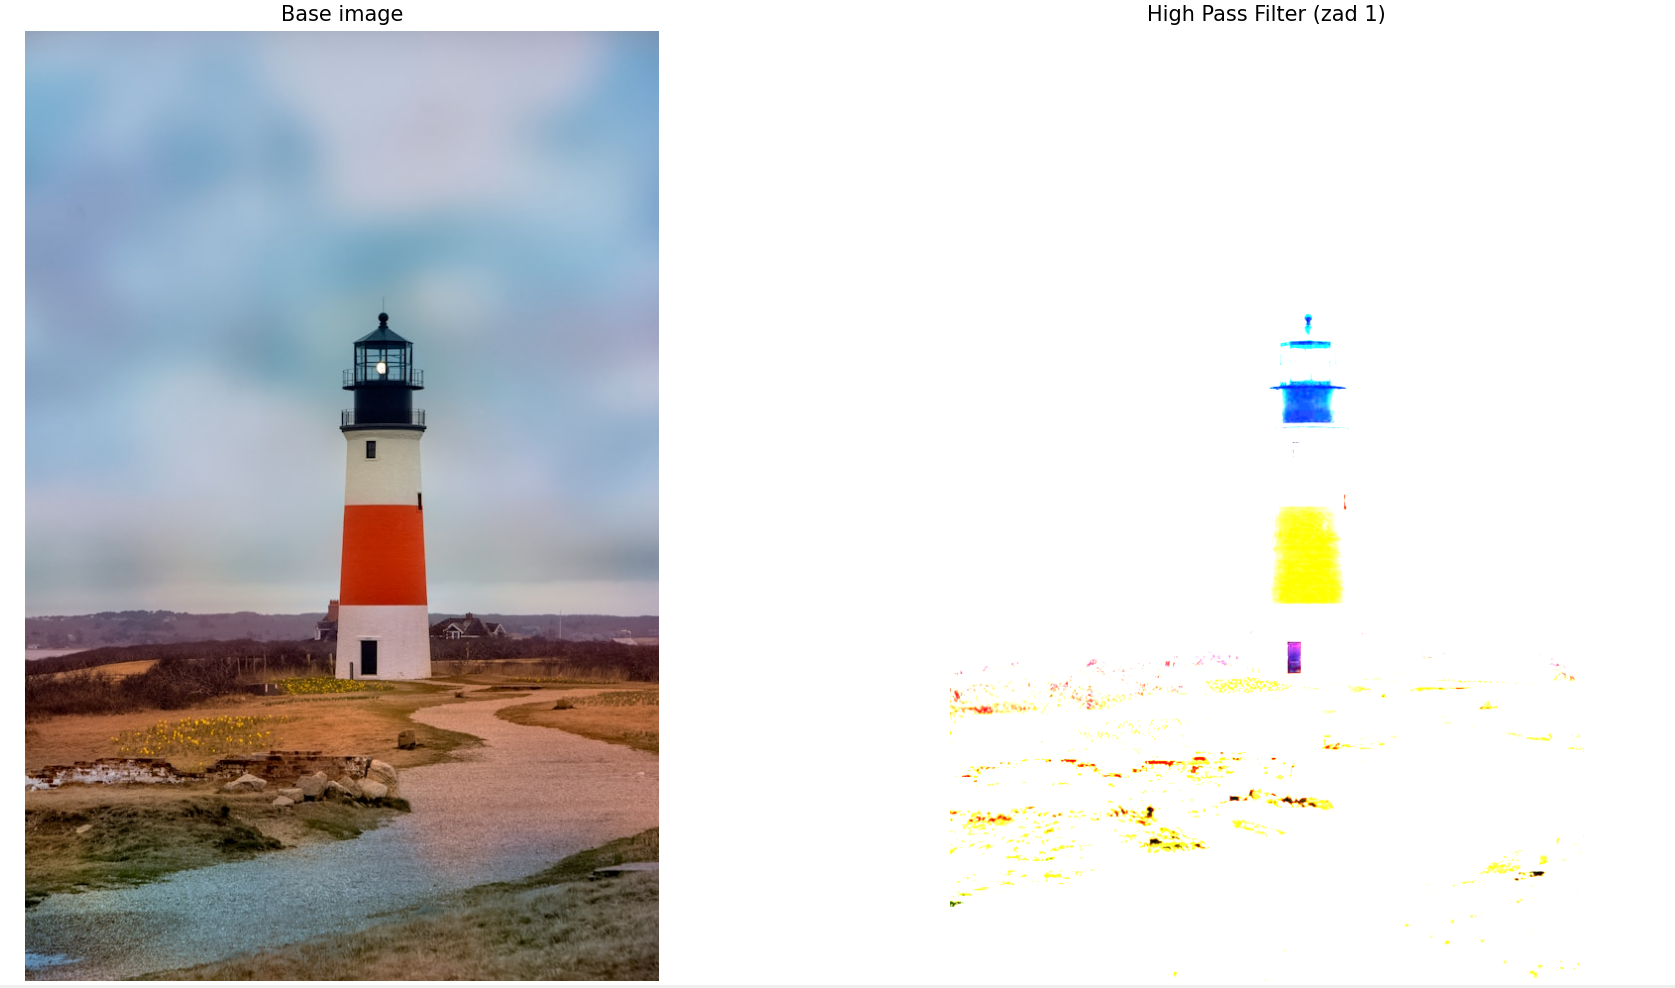
\includegraphics{Img/zad1_1.png}%
        }
        \caption{Otrzymane zdjęcie po nałożeniu maski: $\begin{bmatrix}
                                                            1 & 1 & 1 \\
                                                            1 & 8 & 1 \\
                                                            1 & 1 & 1
                                                        \end{bmatrix}$}
    \end{figure}

    \begin{figure}[H]
        \centering
        \resizebox{\columnwidth}{!}{%
        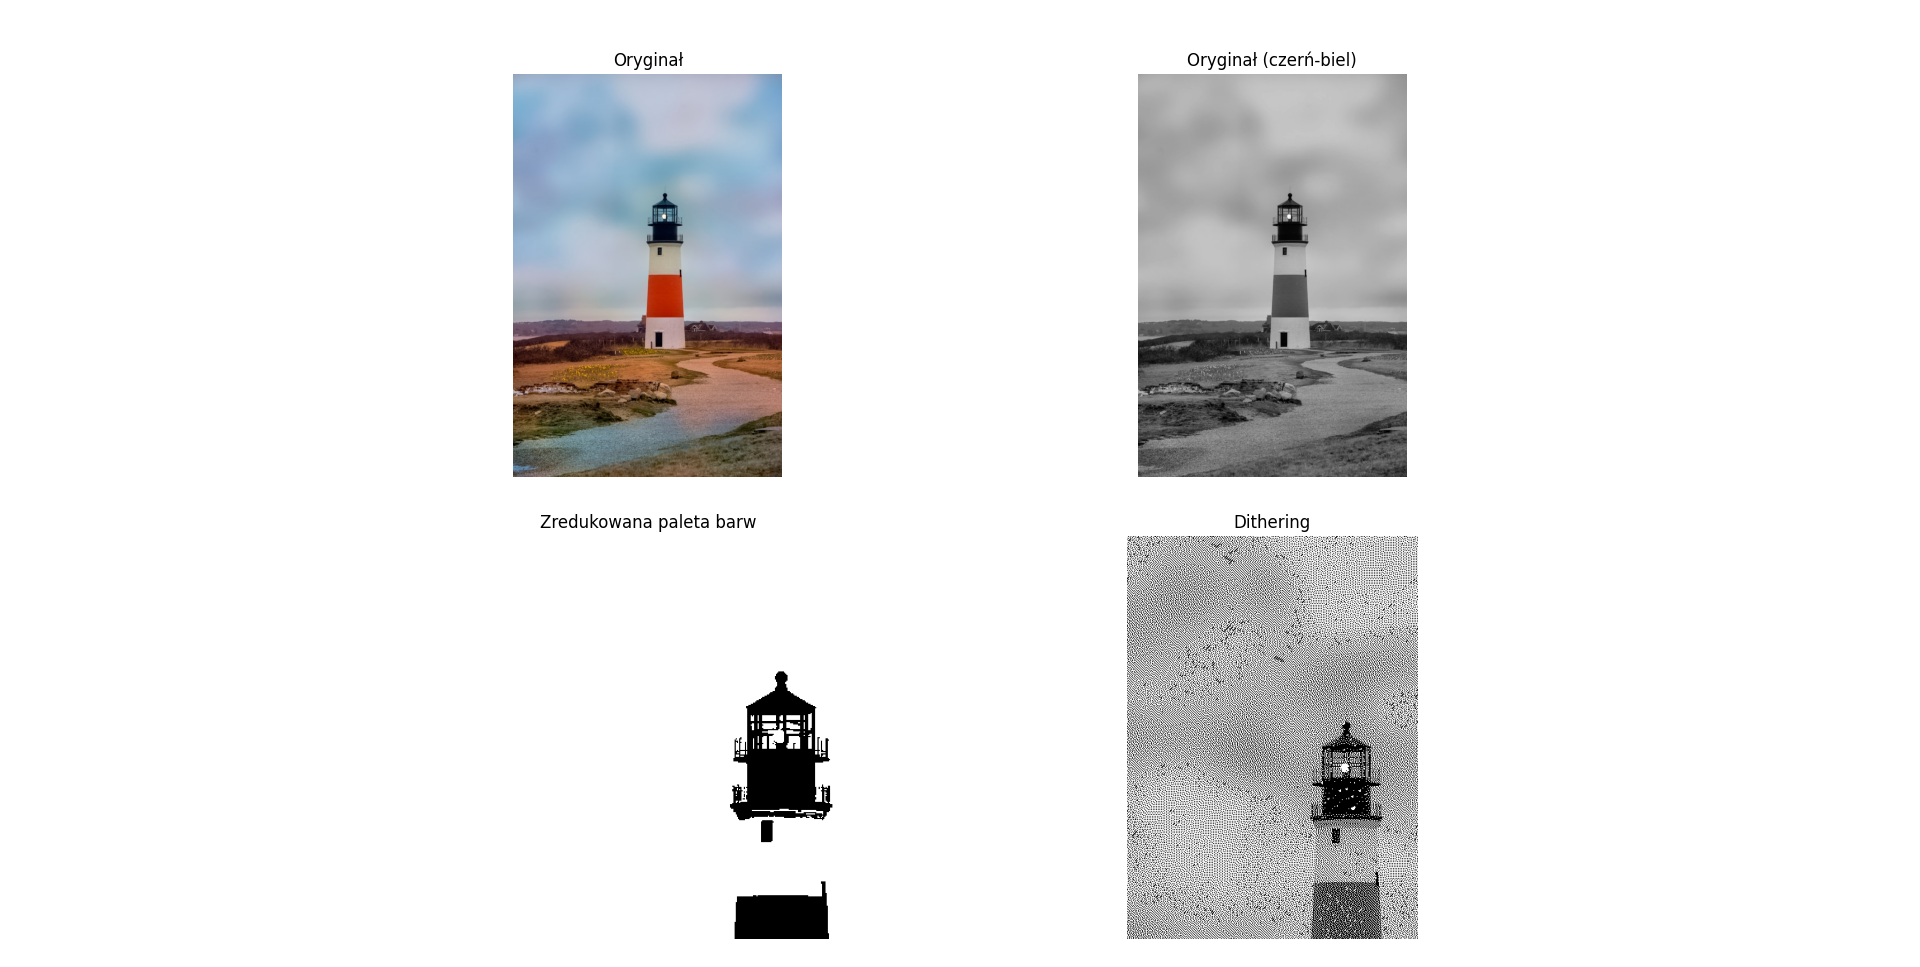
\includegraphics{Img/zad1_2.png}%
        }
        \caption{Otrzymane zdjęcie po nałożeniu maski: }
    \end{figure}

    $\begin{bmatrix}
        0 & 1/21 & 1/21 & 1/21 & 0 \\
        1/21 & 1/21 & 1/21 & 1/21 & 1/21 \\
        1/21 & 1/21 & 1/21 & 1/21 & 1/21 \\
        1/21 & 1/21 & 1/21 & 1/21 & 1/21 \\
        0 & 1/21 & 1/21 & 1/21 & 0 
    \end{bmatrix}$



\section{Zadanie drugie}
\section{Zadanie trzecie}




\bibliographystyle{plainnat}
\bibliography{TexBase/Bibliography.bib}

\end{document}